
% this file is called up by thesis.tex
% content in this file will be fed into the main document

%: ----------------------- introduction file header -----------------------
\chapter{Introduction and related work}

% the code below specifies where the figures are stored
\graphicspath{{1_introduction/}}

\begin{abstract}{Résumé}

L'architecture spatiale et temporelle du génome joue un rôle important dans
beaucoup de fonctions génomiques, mais est cependant à l'heure actuelle peu
comprise. Le développement récent du protocol Hi-C, qui permet en une seule
expérience de mesurer les fréquences d'interactions entre paire de loci sur
tout le génome, ouvre la porte à une étude plus systématique de la structure
tridimensionnelle du génome. Dans ce chapitre, nous introduisons les concepts
sous-jacents à la capture de la conformation des chromosomes, la structure de
l'ADN et aux méthodes d'inférence de l'architecture 3D du génome.

\end{abstract}

\begin{abstract}{Abstract}

The spatial and temporal genome architecture is thought to play an important
role in many genomic functions, but is yet poorly understood. Recently, the
development of the Hi-C protocol, which allows in a single experiments to
assess genome wide physical interactions between pairs of loci, has paved the
way for a systematic analysis of the 3D structure of DNA. We aim in this
chapter at providing some background on chromosome conformation capture, the
structure of DNA and the field of 3D architecture inference.

\end{abstract}


\section{Peeking under the hood of genome architecture}

Methods to investigate the 3D structure of the genome fall broadly into two
categories: bio imaging techniques and biochemical protocols. In the first
category, light microscopy allows single cell visualization of specific loci
and enables live cell imaging, sometimes at very high resolution
\citep{cremer:chromosome-2010}. Yet, these techniques limit studies to a very
small number of loci. On the other hand, biochemical protocols, such as
chromosome conformation capture (3C) and its derivatives, enable to measure
physical interaction between DNA fragments \citep{dekker:capturing}, but
performing single cell experiments is troublesome, and tracking live cell
impossible. To understand how DNA fold into a nucleus, one has to jungle
between both technologies. In this thesis, we are mostly interested in
analysing 3C-based datasets.

\subsection{3C, 4C, 5C and Hi-C data}

In recent years, the technique of chromosome conformation capture (3C)
\citep{dekker:capturing}, which identifies physical contacts between different
genomic loci and yields information about their relative spatial distance in
the nucleus, has paved the way for the systematic analysis of the 3D structure
of DNA. 3C techniques and its derivatives are based on 5 experimental steps
\citep{lieberman-aiden:comprehensive, kalhor:genome}.

\begin{itemize}
\item \textbf{Cross-linking} : results in the cross-linking of DNA segments to
proteins and to cross-linking of proteins with each other.
\item \textbf{Restriction digest} A restriction enzyme is added in excess to
the cross-linked DNA. The restriction enzyme will cut the DNA at specific
nucleotide sequences, separating the non-cross-linked DNA from the
cross-linked chromatin. Recognition sequences in DNA differ from each
restriction enzyme, producing different lengths and sequences of strands.
The selection of the restriction enzyme depends on the type of studies
targeted in the experiment.
\item \textbf{Intramolecular Ligation} The third step is an intramolecular
ligation step. DNA fragments are binded together. There are two major types
of ligation junctions: the first is the ligation of two neighboring DNA
fragments, and the second is the junction that is formed when ligating one end
of the fragment to the other end of the same fragment. The latter represents
around 30\% of the junctions formed.
\item \textbf{Reverse Cross-links} The fourth step consists of reversing the
first step: the reversal of cross-links.
\item \textbf{Quantitation} Polymerase chain reaction (PCR) is used to amplify
the DNA copies and to assess the frequencies of the fragments of interest,
which are then sequenced.
\end{itemize}

\begin{figure}
\begin{center}
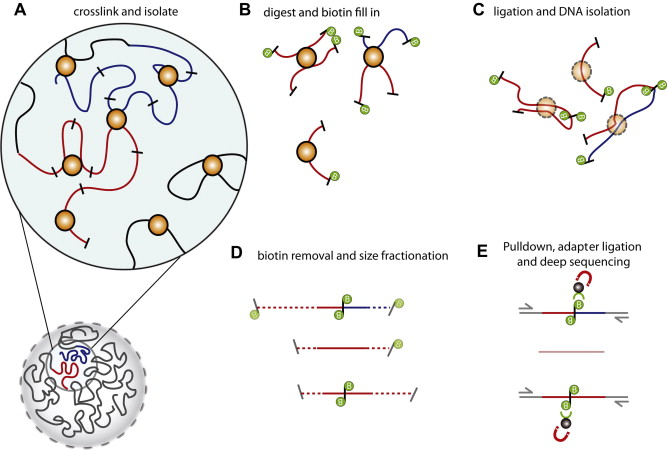
\includegraphics[width=0.8\linewidth]{figures/hic_protocol.png}
\end{center}
\caption{\textbf{Hi-C Protocol.} The procedure relies on cross linking,
restriction enzymes digestions, intra molecular ligation, deproteinization and
deep sequencing. Reads are then aligned to the reference genome, and binned at
$10kb$, $40bk$ or $100kb$ depending on coverage.}
\end{figure}


After paired-end sequencing, each pair of reads can be associated to one
\citep{lieberman-aiden:comprehensive} or several \citep{ay:identifying} DNA
interactions. We can then create a symmetric hollow matrix of integers, for
which entries correspond to the number of paired reads that fall into a bin.
We denote by $C$ the interaction frequency matrix, and $c_{ij}$ the
interaction frequency between locus $i$ and locus $j$.

These protocols are complex, and yield highly biased interaction frequencies
\citep{imakaev:iterative, cournac:normalization, yaffe:probabilistic}.
\citet{imakaev:iterative} proposes a simple iterative method, called ICE, to
normalize the data. In short, the authors assume that the bias of each entry
$c_{ij}$ of the matrix can be written as the product of two biases $\beta_i$
and $\beta_j$ corresponding to biases induced by loci. Hence, we can write
$c_{ij} = \beta_i \beta_j p_{ij}$, where $p_{ij}$ is the probability of locus
$i$ interacting with locus $j$. Thus, $\sum_i p_{ij} = 1$. This is a non convex
optimization problem that can be solved exactly by an iterative process. To
avoid degeneracies, we filter out the top 2\% sparse loci from our entry
matrix before applying ICE. To give an intuition, this method projects each
vector of interactions onto the $\ell_1$ unit ball. In practice, it yields an
expected interaction frequency count: $k p_{ij}$, where $k$ is the mean
interaction frequency.

Thought still quite recent, chromosome conformation capture and its genome
wide derivatives are now widely used to discover how DNA folds in a bunch of
different organisms \citep{duan:three, sexton:three-dimensional,
tanizawa:mapping, ay:three-dimensional}. The challenge is now to increase the
Hi-C resolution, using very large data sets with deeper sequencing
\citep{rao:3d, jin:high-resolution}. As any genome-wide sequencing data, Hi-C
usually requires several millions or billions of paired-end sequencing reads,
depending on genome size and on the desired resolution. Managing these data
thus requires optimized bioinformatics workflows able to extract the contact
frequencies in reasonable computational time and with reasonable storage
requirements. The overall strategy to analyze Hi-C data is converging among
recent studies and summarized in \cite{lajoie:hitchhiker}. Our collaborators
and we have built HiC-Pro, an an easy-to-use and complete pipeline to process
Hi-C data from raw sequencing reads to the normalized contact maps. Once these
processing steps are done, one can finally proceed to the study of genome
organization and DNA folding from Hi-C data in an attempt to unfold the
mysteries of genome architecture.

\section{The study of chromosome organization}

The study of chromosome organization based on contact counts maps broadly
falls into two categories: model-based studies and data-driven studies. The
former methods consider the polymer nature of DNA to leverage the theoretical
and computational work done in statistical physics of polymers to built with
as few assumptions as possible many chromosome conformations. Those chromosome
conformations are then used to compare against experimental data, such as Hi-C
contact counts matrices, in order to iteratively improve the models. These
models offer mechanistical insights into the folding of DNA. The latter
approaches use the experimental data to infer 3D models, by typically minizing
a cost function ensuring the models are as consistent as possible with the
data. These data driven models and analysis are the primary focus of this
thesis.

Though we here review some of the methods used to study and build models, this
is a very incomplete view of a blooming field. \citet{rosa:computational}
provide a more thorough (but again incomplete) overview of computational models
of genome architectures.

\subsection{DNA as a polymer}

Polymer physics divide homopolymers (polymers with identical monomers) into
three main types, which are then extended to build more complex models (1) the
\textit{random coil}, (2) the \textit{swollen coil}, (3) the
\textit{equilibrium polymer}. These polymers are characterized by
relationships such as the one between the size of a polymer subchain $L(s)$ as
a function of its lengths $s$, between the size of the polymer $L(N)$ and the
total length of this polymer $N$, or between the contact probability between
monomers $P(s)$ and the linear distance between monomers $s$. DNA being a
polymer, each pair of nucleic acid forms a monomer, and the distance $s$ is the
genomic distance between two loci.

The \textit{random coil} corresponds to an unconstrained polymer, best
described by a random walk. A \textit{random coil} of length $N$ has an
expected size of $N^{1/2}$, and so has any of its subchain: $L(s) \sim
s^{1/2}$. The contact probability between two monomers is $P(s) \sim
s^{-3/2}$. These relationships lead to a low density polymer, where contact
between monomers is sparse. The modeling of the \textit{random coil} does not
exclude the volume occupied by monomers: when taking in account that monomers
can not occupy the same chain, one obtains a new polymer model known as the
\textit{swollen coil}, best described as a self avoiding random walk. This
type of polymer occupies a larger space: $L(N) \sim N^{\frac{3}{5}}$.

\begin{figure}
\begin{center}
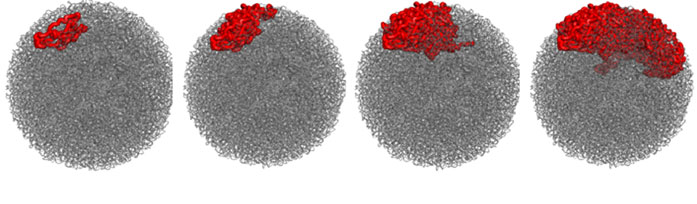
\includegraphics[width=0.8\linewidth]{figures/mirny_fractal.png}
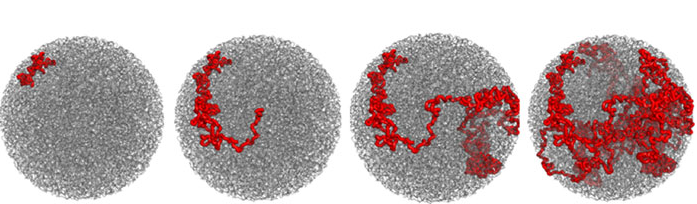
\includegraphics[width=0.8\linewidth]{figures/mirny_equilibrium.png}
\end{center}
\caption{\textbf{Fractal globule versus the equilibrium globule}}{This image
from \citet{mirny:fractal} illustrates the difference between the
\textit{fractal globule} or crumpled globule and the
\textit{equilibrium globule}. In the first row, the
fractal globule's subchain occupes a distinct territory in the nucleus, while
the second row illustrates the equilibrium globule's property to occupy a wide
space in the nucleus.}
\end{figure}

If the polymer is constrained in a small volume, the polymer folds into an
\textit{equilibrium globule} state. This polymer behaves as a random walk,
until it bounces of the boundary of the constrained space, and starts another
random walk inside the confined volume. The expected size of this polymer is
$N^{1/3}$. The size of a subchain of a polymer follows the relationship: $L(s) =
s^{1/2}$ for $s < N^{2/3}$ and constant elsewise: it is the same as a random
coil until it plateaus. The probability of contact between two monomers is
$P(s) = s^{-3/2}$ for $s < N^{2/3}$ and constant elsewise: once again, it is
the same relationship as the random coil, until it becomes constant.
Interestingly, this polymer is uniformely distributed in the constrained
space, and the density of the polymer is independent of the total length $N$
and the volume $V$.

Another interesting polymer behaviour is the \textit{fractal globule}: when
the chain is sufficiently long and the constrained volume sufficiently small,
the polymer forms knotted crumples of increasing sizes. The polymer is then
constrained by the available volume, and other parts of the polymer, which
creates topological constraints forcing the polymer to collapse into crumples.
First proposed by \citet{grosberg:role}, and further analysed by
\citet{mirny:fractal}, the polymer presents interesting properties: the size
of any subchain follows the same law as the equilibrium globule, but without
the plateau: $L(s) \sim s^{1/3}$, and the probability of contact between two
monomers is inversely proportional to the linear distance that separates them:
$P(s) \sim s^{-1}$.


\begin{figure}
\begin{center}
\includegraphics[width=0.7\linewidth]{figures/fig_phd.pdf}
\end{center}
\caption{{\bf Relationship between contact counts and genomic distances}}{
Average contact counts as a function of genomic distance for \textit{S.
cerevisiae} \citep{duan:three-dimensional},
\textit{D. melanogaster} \citep{sexton:three-dimensional} and chr~1 of the
KBM7 human cell line \citep{rao:3d}. \textit{S. cerevisiae}'s genome behaves
as a \textit{equilibrium globule},
while \citet{sexton:three-dimensional}'s \textit{D.
melanogaster} and \citet{rao:3d}'s KBM7 datasets display relationships of the
\textit{fractal crumpled globule}. Notice that \textit{S. cerevisiae}'s
average contact counts decreases more quickly with the genomic distance than
\textit{D. melanogaster}'s and KBM7's.
}
\label{fig:hic_relationships}
\end{figure}

Now that we have briefly summarized the different theoritical behaviour of
polymers DNA can adopt, let us have a closer look at the relationships we
observe in the contact counts maps. We can observe that organism fall into two
categories: the first group, composed of small genomes such as \textit{S.
cerevisae}, \textit{P. falciparum}, behaves as an \textit{equilibrium globule}
coil, while the second group, composed of large genomes such as mammifer
genomes and \textit{A. thaliana} \textit{D. drosophilae}, exhibit properties
of \textit{fractal globules}.

\subsection{The inference of DNA three-dimensional models}


Several techniques have been developed to infer three-dimensional models of
the genome from interaction counts data. They fall into three categories: the
first finds an average structure by optimizing an objective function as
\citep{tanizawa:mapping, duan:three, ben-elazar:spatial}. The
second samples local minima from a optimization problem leading to the study
of the population of local minima \citep{bau:three-dimensional}. The last
samples the posterior distribution \citep{rousseau:three}.

\citet{tanizawa:mapping} model the 3D genome of the fission yeast (3
chromosomes) by a string of $622$ beads, each bead $x_i$ being the center of a
$20$kb section. The first step was to infer physical distances $\delta_{ij}$
from frequency interactions. They studied eighteen pairs of genes using FISH
measurements, and fitted the Hi-C data on the distances with a non linear
regression curve. The second step was to compute the coordinates of the beads,
such that the distances between the beads matches the inferred physical
distances to the best, with additional biological motivated constraints.

\citet{duan:three} converts the interaction frequencies into distances by
examining the relationship between interaction frequencies and genomic
distances. Then, a multidimensional scaling (MDS) is used to place each bead
so that the wish distances are respected as well as possible.

\citet{tanizawa:mapping} and \citet{duan:three} optimizes a problem of the
form:
\begin{equation*}
\renewcommand{\arraystretch}{2}
\begin{array}{ccll}
\underset{x_1,\ldots, x_n}{\text{minimize}} & &
\underset{i<j\leq n}{\sum} \big(\|x_i - x_j\|_2 - \delta_{ij}\big)^2 &\\
\text{subject to}
& & \text{biological motivated non convex constraints.}
\end{array}
\end{equation*}

\citet{tanizawa:mapping} published one solution, but did not mention the non
convexity of the problem. Hence, we assume they seeked the best local minimum
\citet{duan:three} ran the optimization process 30 times, and, observing the
obtained solutions, found that they did not differ much. No formal study was
done to compare the solutions.

\citet{lesne:3d} proposes a classical MDS algorithm \textit{ShRec3D} as follows:
(1.) construct a graph whose vertices are the loci assessed in the Hi-C
experiment, and the weights of vertices inversely proportional to the contact
counts (2.) compute a matrix of shortest path between pairs of loci which we
denote by the ``distance`` matrix (3.) apply a classical MDS on this distance
matrix. This yields a fast algorithm for inferring a consensus algorithm.

\citet{ben-elazar:spatial} formulated a non metric multidimensional scaling
optimization problem. They first filtered the interaction count matrix so that
remained only the most significant interactions. They then interpolated the
missing values to obtain a smooth, symmetric, positive definite matrix.

\citet{bau:three-dimensional} used IMP (Integrative Modeling Platform), also
used in nuclear magnetic resonance (NMR) microscopy to construct a 3D model of
the $\alpha$-globin module. Chromosomes are represented by beads, each beads
linked by restraining oscillators. IMP seeks a solution at the equilibrium of
those beads. Three types of restraints are used: the first  corresponds to
harmonic oscillators, with strengths inversely proportional to the 5C
score, computed from the interaction frequencies. The second ensures that two
beads cannot be too close to each other. The third ensure that two consecutive
beads cannot be separated too much. The last two springs have strength only
when the constraints are not fulfilled. The optimization of this problem
yields different configuration with similar IMP scores. A population of 50000
structures was computed. The 10000 structures with the smaller objective
function were then chosen as the population of local minima to be studied.

\citet{rousseau:three} and \citet{hu:bayesian} both describe a formal
probabilistic model of interaction frequencies and their relationship with
physical distances. They then use a Markov Chain Monte Carlo sampling
procedure to produce an ensemble of 3D structures consistant with the contact
count data.

\citet{tjong:physical} constructs a very simple model of the budding yeast
{\em S. cerevisiae} by modeling chromosomes
as a flexible fiber, and using additional biologically motivated constraints,
such as the positioning of centromeres and telomeres, they formulate an
optimization problem. Generating $200000$ feasible structures, they show that
Hi-C data can be fully explained by this very simple model.

\citet{wong:how} models the budding yeasts chromosomes a semi-flexible fiber
constrained in a nucleus, and applies 4 sequences specific forces on this
fiber to obtain certain properties: (1) centromeres are attached to a single
point of the nucleus by a segment; (2) telomeres are subjected to an outward
force, that pushes them towards the nuclear membrane; (3) rDNA is thicken; (4)
apply a random brownian movement. This models recovers many of the known
hallmarks of the 3D architecture of {\em S. cerevisiae}.

\citet{nagano:single-cell} and \citet{paulsen:manifold} both proposes methods
to infer 3D structures from single-cell Hi-C data. The first is a constraint
based modelisation: the structure is modeled as a flexible fiber as in
\citet{tjong:physical}, but beads are constraint to be in contact when an
interaction is observed in the single-cell contact map.
\citet{paulsen:manifold} formulates a \textit{manifold based optimization},
where a low rank psd matrix (and thus a distance matrix) is optimized to be as
close as possible to the sparse contact count matrix. Applying classical MDS
on this low rank psd matrix then yields a 3D model of the genome.

\begin{table}[ht!]
\caption{\bf A comparison of 3D inference methods}
\begin{center}
\small
\begin{tabular}{rlccccc}
\hline
\multirow{2}{*}{\emph{Publication}} & \multirow{2}{*}{\emph{Name}} &
\multirow{2}{*}{\emph{Consensus}} & \multirow{2}{*}{\emph{Population}}
&\multirow{2}{*}{\emph{MDS-based}} & \emph{Statistical} &
\multirow{2}{*}{\emph{Available}} \\
& & & & & \emph{model} & \\
\hline
\citet{duan:three} &  & x & & x & & x \\
\citet{tanizawa:mapping} & & x & & x & & \\
\citet{ay:three-dimensional} & & x & & x & & \\
\citet{ben-elazar:spatial} & & x & & x & & x \\
\citet{varoquaux:statistical} & Pastis & x & & & x & x\\
\citet{bau:three-dimensional} & & & x & & & \\
\citet{umbarger:three-dimensional} & & x & & & &\\
\citet{zhang:inference} & chromSDE & x & & x & & x\\
\citet{rousseau:three} & & & x & & x & x\\
\citet{hu:bayesian} & Bach & x & x & & x & x\\
\citet{kalhor:genome} & & & x & & &\\
%\citet{tokuda:dynamical} & & & & & &\\
\citet{wong:predictive} & & & x & & & \\
%\citet{gehlen:chromosome} & & & & & &\\
\citet{lesne:3d} & ShRec3D & x & & x & & x \\
\citet{trieu:large} & & x & & & & \\
\end{tabular}
\end{center}
\end{table}


\section{Long range interactions}


Thought mostly and initially used to study DNA folding, contact counts maps
have recently been re-purposed for diverse applications: \textit{de novo}
genome assembly \citep{burton:chromosome, kaplan:high-throughput},
deconvolution of metagenomic samples \citep{burton:species-level,
beitel:strain}, and genome annotation \citep{marie-nelly:filling,
varoquaux:accurate}.

\subsection{\textit{De novo} genome assembly, haplotype resolution and
metagenomic sample deconvolution}

\textit{De novo} genome assembly is the task of assembling many short DNA
reads into a whole genome. These short DNA reads can be assembled into short
contigs but the process of joining short contigs into larger scaffolds is
often made difficult due to the presence of repetitive sequences. Despite
improvements in sequencing technology and thus the sequencing of longer reads,
filling the gaps caused by these repetitive sequences in complex genome
remains difficult. \citet{burton:chromosome} and
\citet{kaplan:high-throughput} proposes to use the massive amount of DNA
sequences produced by Hi-C to first assemble short contigs, and rely on
contact counts informations between contigs to attempt to place them one
relatively to the other. Indeed, the more two contigs interact, the closer in
terms of genomic distances they should be (with the proper normalization in
contig lengths, GC-content, mappability and so on). The contact count matrix
of the ordered contigs (the "normal" contact count map) is simply a
permutation of rows and columns of the contact count matrix of the unordered
set of contigs. Assembling the genome can thus be seen as reordering rows and
columns to obtain a suitable Hi-C contact count matrix, smooth and with a
strong diagonal. \citet{burton:chromosome} proposes to first cluster contigs
into groups that belong to the same chromosomes, then create a graph where
each node is a contig, and vertex represents interactions of weight contact
counts. They then apply a minimum spanning tree algorithm to identify a path
in the graph corresponding to adjacent contigs. \citet{kaplan:high-throughput}
and \citet{marie-nelly:high-quality} both formulate the task as finding a
permutation of rows and columns to maximize a likelihood. As finding a
permutation matrix is a NP-hard problem, they use heuristic to simplify the
optimization problem.

Mammifer genomes contain two copies of each chromosomes, which themselves hold
specific single nucleotide polymorphisme (SNP). It is sometimes interesting to
identify whether SNPs or mutations are held on the same copy of the
chromosome. The task of identifying which SNP belongs to which chromosome is
known as resolving the haplotype. \citet{selvaraj:whole-genome}
proposes a very similar idea as
before, which is that reads containing SNPs on the same homologous chromosomes
interact more than SNPs on the other homologous chromosome. It is thus
possible to use contact count information between reads in order to determine
to which homologous chromosomes SNPs belong and resolve the haplotype.

Microbiomes contain an ensemble of very small organisms in different
abundances. Traditionnal technics to identify which organisms is in a
metagenomic sample rely on deep sequencing to produce millions of short DNA
reads. These reads are then either aligned on a reference genome or used as
input of a supervised learning algorithm (Kevin) to identify which organisms
are in the sample, and in which abundance. Both of these
methods need a priori knowledge of the community's composition. Recently,
\citet{burton:species-level} and \citet{marbouty:metagenomic} use shotgun
sequencing and Hi-C contact counts to determine which contigs belong to which
organisms. Once again, the idea is very similar as before: contigs from the
same organism interact amongst each other the most. Thus, a clustering
algorithm that takes as input a similarity matrix (the contact counts) groups
contigs from the same organism together. Once the organism's contigs are
identified, one can use technics as described before to scaffold contigs
together, and therefore in a single experiment do \textit{de novo} sequencing
of many organisms, and find the composition and abundance of a metagenomic
samples.

All these applications are based on a very simple and elegant idea that
contact counts map hold information on the contiguity of chromosomes which can
be leverage for various tasks.

\subsection{Genome annotations and centromeres identification}

The last unusual application of Hi-C data is the annotation of genomes, and
more specifically the detection of highly colocolized elements that are
elsewise difficult to annotate. In particular, centromeres have proven
difficult to precisely identify in many species, including highly studied and
used yeasts species. Centromeres, essential for proper chromosome segregation,
have the property of clustering in 3D, and thus have very specific signal
patterns in Hi-C data. \citet{marie-nelly:filling} proposed to annotate
centromeric regions by detecting these very specific patterns in the contact
maps of yeast species.

\section{Contributions of the thesis}

This thesis brings several contributions to the fields of analyzing Hi-C data.
We now review them, following the organization of the manuscript (and not in
chronological order of publication).

\begin{itemize}

\item Chapter \ref{chap:statistical} presents a novel, stable and robust
statistical method for inferring a consensus 3D model of the genome. We model
contact counts as a Poisson distribution where the 3D structure is a latent
variable, and formulate the inference problem as maximizing the likelihood. We
show both on generated and real Hi-C data that our method is more accurate,
stable and robust than previous methods. \footnote{Our method \textit{Pastis}
is available as a free and opensource software at
\url{http://cbio.ensmp.fr/pastis}}

\item Chapter \ref{chap:plasmodium} studies the 3D architecture of the
parasite {\em P. falciparum} during its erythrocytic cycle and its links with
gene expression. We assayed the genome architecture of the parasite at three
time points to obtain high resolution contact maps which we used to construct
consensus 3D models. The resulting models showed that {\em P. falciparum}'s
genome is folded in a complex architecture, that cannot be explained by a
simple volume exclusion model due to the strong co-clustering of many genomic
elements in the nucleus. We observe a strong link between chromatin structure
and gene expression, in particular reduced expression of genes located in
spatial proximity to the repressive subtelomeric center and colocalization of
distinct groups of parasite-specific genes with coordinated expression
profiles. Overall, our results show that the 3D structure of the parasite is
strongly correlated with gene expression during the erythrocytic cycle. This
work has been done in collaboration with Noble lab and Le Roch lab. My
contribution were (1) the 3D modeling of the genome using MDS-like approaches,
(2) the comparison to the volume exclusion modeling and (3) finding the link
between gene expression profiles and the 3D models using kernel CCA.

\item Chapter \ref{chap:centurion} presents work done while I was visiting
Noble lab, in collaboration with Dunham lab and Shendure lab. We proposed a
novel method to jointly identify yeasts centromeres from Hi-C data, using the
property centromeres have to strongly colocolize in the nucleus and thus to
create a specific pattern in the contact counts maps. Our method,
\textit{Centurion}, outperforms a previous published method by performing a
joint optimization and using a better strategy to initialize the optimization.
We show that \textit{Centurion} is very accurate and stable both on high and
low coverage datasets. \footnote{Our method \textit{Centurion} is available as
a free and opensource software at \url{http://cbio.ensmp.fr/centurion}}
\end{itemize}
